\chapter{Pereaksi Organomagnesium}\label{ch:b1:organomagnesium}

Kebanyakan molekul organik yang berguna mempunyai lebih banyak atom
karbon daripada bahan awal murah mana pun, dan persoalan utama sintesis
adalah menyambung dua kerangka karbon melalui ikatan C--C yang baru.
Dalam senyawa karbon, karbon hampir selalu merupakan pihak yang miskin
elektron dalam sebuah ikatan --- dengan oksigen, dengan halogen --- dan
dua karbon yang miskin elektron tidak saling bereaksi. Menjelang awal
abad kedua puluh, sebuah pereaksi yang dibuat dalam satu labu dari
haloalkana dan magnesium membalik keadaan ini: karbonnya kaya elektron,
sebuah \omterm{def:b1:electronic-effects:nucleophile}{nukleofil} yang menyerang karbon gugus karbonil. Dengan pereaksi
itu, alkohol dengan kerangka hampir apa pun dapat dibangun dari
potongan-potongan yang lebih kecil. Bab ini memperlihatkan cara pereaksi
itu dibuat, mengapa pereaksi itu memerlukan labu yang benar-benar
kering, pada apa ia beradisi, dan cara merencanakan sintesis dengannya.

\begin{recall}
\omterm{def:b1:periodicity:electronegativity}{Keelektronegatifan} (\cref{ch:b1:periodicity}); asam dan \omterm{def:b1:lewis-resonance-vsepr:lewis-acid}{basa Lewis} serta
\omterm{def:b1:lewis-resonance-vsepr:lewis-acid}{ikatan datif} (\cref{ch:b1:lewis-resonance-vsepr}); \omterm{def:b1:electronic-effects:nucleophile}{nukleofil}, \omterm{def:b1:electronic-effects:nucleophile}{elektrofil},
\omterm{def:b1:electronic-effects:curly-arrow}{panah lengkung}, dan skala $\mathrm{p}K_a$ spesies organik
(\cref{ch:b1:electronic-effects}); kelas sebuah alkohol (primer,
sekunder, tersier) mengikuti kelas karbonnya.
\end{recall}

\section{Membuat pereaksi Grignard}

\begin{definition}[Senyawa organologam, pereaksi Grignard]\label{def:b1:organomagnesium:organometallic}
\emph{Senyawa organologam}\index{senyawa organologam} mengandung
sedikitnya satu ikatan karbon--logam. \emph{Senyawa
organomagnesium}\index{senyawa organomagnesium} mempunyai ikatan C--Mg;
\emph{pereaksi Grignard}\index{pereaksi Grignard} \ce{RMgX} (X = Cl, Br,
I), yang dibuat dari haloalkana atau haloarena dan magnesium dalam eter,
\ce{R-X + Mg -> R-MgX}, adalah yang paling umum.
\end{definition}

Magnesium menyisipkan dirinya ke dalam ikatan C--X. Eter itu bukan
pelarut yang pasif: magnesium dalam \ce{RMgX} hanya dikelilingi empat
\omterm{def:b1:quantum-numbers:configuration}{elektron valensi}, dan dua molekul eter memberinya \omterm{def:b1:lewis-resonance-vsepr:lewis}{pasangan elektron
bebasnya}, sehingga oktetnya lengkap dan pereaksi itu tetap larut.

\begin{omfigure}
\begin{tikzpicture}[font=\small]
  \node (mg) at (0,0) {Mg};
  \node (r) at (-1.5,0) {R};
  \node (x) at (1.5,0) {Br};
  \node (o1) at (0,1.45) {O};
  \node (o2) at (0,-1.45) {O};
  \draw[thick] (r) -- (mg) -- (x);
  \draw[thick, ->, omDef] (o1) -- (mg);
  \draw[thick, ->, omDef] (o2) -- (mg);
  \draw (o1) -- ++(-0.8,0.45) node[left] {\ce{CH3CH2}};
  \draw (o1) -- ++(0.8,0.45) node[right] {\ce{CH2CH3}};
  \draw (o2) -- ++(-0.8,-0.45) node[left] {\ce{CH3CH2}};
  \draw (o2) -- ++(0.8,-0.45) node[right] {\ce{CH2CH3}};
  \node[align=left, anchor=west] at (3.2,0) {dua molekul eter masing-masing\\memberikan sepasang elektron bebas (biru):\\magnesium tetrahedral,\\sebuah oktet elektron};
\end{tikzpicture}

{\small \omterm{def:b1:organomagnesium:organometallic}{Pereaksi Grignard} dalam etoksietana (dietil eter). Ikatan-ikatan
datif oksigen--magnesium menjelaskan mengapa pereaksi itu hanya
terbentuk dalam eter atau \omterm{def:b1:lewis-resonance-vsepr:lewis-acid}{basa Lewis} yang serupa.}
\end{omfigure}

\begin{method}[Membuat pereaksi Grignard]\label{met:b1:organomagnesium:prepare}
\begin{enumerate}
  \item Keringkan semua alat gelas dalam oven; pasang tabung pengering
        berisi kalsium klorida pada kondensor; gunakan eter anhidrat.
  \item Masukkan serutan magnesium dan sedikit eter ke dalam labu leher
        tiga yang dilengkapi kondensor, corong tetes, dan pengaduk.
  \item Tambahkan sebagian kecil halidanya; ketika reaksi mulai
        (kekeruhan, eter mendidih perlahan), tambahkan sisanya tetes demi
        tetes dengan laju yang menjaga refluks yang perlahan.
  \item Gunakan larutan itu segera, dalam alat kering yang sama.
\end{enumerate}
\end{method}

\begin{omfigure}
\begin{tikzpicture}[font=\small]
  \pic at (0,-0.05) {stirrer};
  \pic (f) at (0,0.05) {threeneck={0.35}{omDef!14}};
  \pic at (f-c) {condenser};
  \pic at ($(f-c)+(0,3.2)$) {guardtube};
  \pic[rotate=25] at (f-l) {dropfunnel={0.5}{orange!20}};
  \fill[black!45, rotate around={-25:(f-r)}] ($(f-r)+(-0.17,0)$) rectangle ++(0.34,0.3);
  \draw[->] (2.4,0.9) node[right] {serutan Mg dalam eter kering} -- (0.6,0.6);
  \draw[->] (-3.0,3.9) node[left, align=right] {halida dalam eter,\\ditambahkan tetes demi tetes} -- (-1.8,3.4);
  \draw[->] (1.8,5.3) node[right] {kondensor (air)} -- (0.45,4.8);
  \draw[->] (1.8,6.6) node[right] {tabung pengering kalsium klorida} -- (0.3,6.4);
  \draw[->] (2.4,-0.2) node[right] {pengaduk magnetik} -- (1.3,-0.2);
\end{tikzpicture}

{\small Alat untuk reaksi Grignard: segala sesuatu yang dapat dicapai
udara dikeringkan. Uap air dari udara dihentikan oleh tabung pengering;
kondensor mengembalikan eter yang mendidih ke dalam labu.}
\end{omfigure}

\begin{inthelab}[Reaksi yang harus dimulai]
Pembuatan \omterm{def:b1:organomagnesium:organometallic}{pereaksi Grignard} kadang-kadang menolak dimulai: magnesiumnya
tertutup lapisan oksida. Menghancurkan sebuah serutan dengan batang kaca,
menambahkan sebutir \omterm{def:b1:crystals-metals:crystal}{kristal} iodin, atau memanaskan labu secara setempat
membuka permukaan logam yang segar. Setelah dimulai, reaksinya eksoterm
dan eter mendidih dengan sendirinya; penambahannya lalu diperlambat agar
tidak meluap. Etoksietana mendidih pada \qty{35}{\celsius} dan uapnya
sangat mudah menyala: tidak boleh ada nyala api di mana pun di dalam
laboratorium, dan penangas es selalu siap di dekatnya.
% ledger: bp:diethylether
\end{inthelab}

\section{Basa kuat sekaligus nukleofil}

\begin{definition}[Inversi polaritas]\label{def:b1:organomagnesium:umpolung}
\omterm{def:b1:periodicity:electronegativity}{Keelektronegatifan} magnesium (1.31) jauh lebih rendah daripada
\omterm{def:b1:periodicity:electronegativity}{keelektronegatifan} karbon (2.55): dalam \ce{R-MgX} ikatan C--Mg
terpolarisasi dengan ujung negatif pada karbon, yang berperilaku sebagai
\omterm{def:b1:electronic-effects:intermediates}{karbanion}. Dalam halida \ce{R-X} karbon yang sama bermuatan positif
(X: 2.96 untuk Br). Mengubah karbon yang elektrofilik menjadi karbon yang
nukleofilik adalah \emph{inversi polaritas}\index{inversi polaritas}.
% ledger: en:Mg, en:C, en:Br
\end{definition}

\begin{proposition}[Pereaksi Grignard dirusak oleh hidrogen yang asam]\label{prop:b1:organomagnesium:base}
\omterm{def:b1:organomagnesium:organometallic}{Pereaksi Grignard} bereaksi secara \omterm{def:b1:extent-q-and-k:quantitative}{kuantitatif} dengan air, alkohol, asam
karboksilat, amina yang mempunyai ikatan N--H, dan alkuna terminal,
menghasilkan alkana \ce{R-H}: \ce{RMgX + H2O -> R-H + Mg(OH)X}.
\end{proposition}

\begin{proof}
Karbon yang mirip \omterm{def:b1:electronic-effects:intermediates}{karbanion} itu adalah basa pasangan \ce{R-H}/\ce{R^-},
dan alkana adalah asam organik yang jauh paling lemah: tidak ada proton
yang dapat diukur lepas darinya di dalam air, tempat hidroksida adalah
basa terkuat yang dapat ada (\cref{ch:b1:predominant-reaction},
perataan). Setiap asam dalam daftar itu jauh lebih kuat, dan perpindahan
proton ke \ce{R^-} mempunyai tetapan yang sangat besar: perpindahan itu
sempurna dan cepat.
\end{proof}

Inilah alasan alat yang kering: setetes air merusak pereaksi dalam
jumlah yang sama. Jika dijadikan keuntungan, \ce{CH3CH2MgBr + D2O}
menempatkan sebuah atom deuterium tepat di tempat brom sebelumnya.

\section{Adisi pada senyawa karbonil dan karbon dioksida}

Karbon gugus C=O bersifat elektrofilik (\cref{ch:b1:electronic-effects}).
\omterm{def:b1:organomagnesium:organometallic}{Pereaksi Grignard} mengadisikan gugus R-nya pada karbon itu, dengan
pasangan $\pi$ C=O berpindah ke oksigen; pengolahan akhir dengan asam
lalu memprotonasi alkoksidanya.

\begin{omfigure}
\setchemfig{atom sep=2.1em}
\schemestart
\chemfig{@{r}R-[@{rm}]MgBr}
\+
\chemfig{@{cc}C(-[:150]R')(-[:210]R'')=[@{co}]@{o}O}
\arrow{->}
\chemfig{C(-[:150]R')(-[:210]R'')(-[2]R)-O^{-}}
\chemfig{\phantom{.}}\chemfig{^{+}MgBr}
\arrow{->[\ce{H3O+}]}
\chemfig{C(-[:150]R')(-[:210]R'')(-[2]R)-OH}
\schemestop
\chemmove{\draw[->, thick, shorten <=2pt, shorten >=2pt](rm) .. controls +(70:9mm) and +(180:7mm) .. (cc);
          \draw[->, thick, shorten <=2pt, shorten >=2pt](co) .. controls +(90:6mm) and +(90:6mm) .. (o);}
\par\vspace{6pt}

{\small Adisi \omterm{def:b1:organomagnesium:organometallic}{pereaksi Grignard} pada keton (atau aldehida,
$\mathrm{R''} = \mathrm{H}$): pasangan C--Mg membentuk ikatan C--C baru
sementara pasangan $\pi$ C=O berpindah ke oksigen; magnesium alkoksida
diprotonasi oleh asam encer pada tahap tersendiri.}
\end{omfigure}

\begin{proposition}[Alkohol dari senyawa karbonil]\label{prop:b1:organomagnesium:carbonyl-addition}
Sesudah pengolahan akhir dengan asam, \omterm{def:b1:organomagnesium:organometallic}{pereaksi Grignard} \ce{RMgX}
menghasilkan: dengan metanal, alkohol primer \ce{RCH2OH}; dengan aldehida
lain $\mathrm{R'CHO}$, alkohol sekunder $\mathrm{RR'CHOH}$; dengan keton
$\mathrm{R'COR''}$, alkohol tersier $\mathrm{RR'R''COH}$. Ikatan C--C
yang baru menyambung R dengan bekas karbon karbonil.
\end{proposition}

\begin{proof}
Karbon karbonil mempertahankan kedua substituennya dan memperoleh R dan
sebuah OH (dari oksigen alkoksida): metanal membawa dua H, aldehida satu
H dan satu gugus karbon, keton dua gugus karbon. Kelas alkohol adalah
banyaknya gugus karbon pada karbon itu: satu, dua, atau tiga.
\end{proof}

\begin{proposition}[Asam karboksilat dari karbon dioksida]\label{prop:b1:organomagnesium:co2}
\omterm{def:b1:organomagnesium:organometallic}{Pereaksi Grignard} yang dituangkan ke atas karbon dioksida padat
menghasilkan, sesudah pengasaman, asam karboksilat \ce{RCOOH} yang
karbonnya bertambah satu: \ce{RMgX + CO2 -> RCOOMgX}, lalu
\ce{RCOOMgX + H3O+ -> RCOOH + Mg^2+ + X- + H2O}.
\end{proposition}

\begin{proof}
\ce{CO2} adalah senyawa karbonil yang karbonnya diserang seperti karbon
keton; karboksilat yang terbentuk terlalu tidak reaktif untuk
mengadisikan gugus R kedua pada kondisi ini (karbonil yang bermuatan
negatif adalah \omterm{def:b1:electronic-effects:nucleophile}{elektrofil} yang buruk). Asam memprotonasinya.
\end{proof}

\section{Membangun kerangka karbon}

\begin{method}[Merencanakan sebuah alkohol]\label{met:b1:organomagnesium:plan-alcohol}
\begin{enumerate}
  \item Temukan karbon yang membawa OH dalam alkohol sasaran.
  \item Pilihlah salah satu gugus karbonnya sebagai R (gugus itu akan
        berasal dari \omterm{def:b1:organomagnesium:organometallic}{pereaksi Grignard}, yang dibuat dari \ce{R-Br});
        sisa molekulnya, dengan karbon itu sebagai C=O, adalah pasangan
        karbonilnya.
  \item Daftarkan pilihan-pilihan yang mungkin (satu per gugus karbon)
        dan utamakan pilihan dengan pereaksi yang sederhana dan tersedia.
  \item Periksalah bahwa tidak ada pihak yang membawa hidrogen asam atau
        gugus karbonil kedua yang juga akan bereaksi.
\end{enumerate}
\end{method}

\begin{example}[2-Fenilbutan-2-ol]\label{ex:b1:organomagnesium:plan}
Karbon yang membawa OH membawa gugus fenil, metil, dan etil. Tiga
pilihan: fenilmagnesium bromida dengan butan-2-on; metilmagnesium bromida
dengan 1-fenilpropan-1-on; etilmagnesium bromida dengan 1-feniletan-1-on
(asetofenon). Ketiganya berhasil; yang terakhir memakai dua pereaksi
yang paling umum.
\end{example}

\begin{history}[Victor Grignard]
\begin{minipage}[t]{0.2\linewidth}\vspace{0pt}
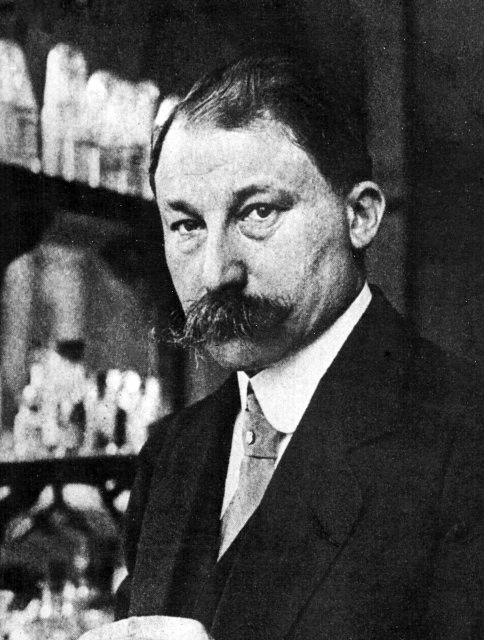
\includegraphics[width=\linewidth]{images/book2/grignard.jpg}
\end{minipage}\hfill
\begin{minipage}[t]{0.76\linewidth}\vspace{0pt}
Pereaksi ini menyandang nama Victor Grignard, yang, sebagai mahasiswa
doktoral menjelang awal abad kedua puluh, menemukan bahwa magnesium larut
dalam larutan haloalkana dalam eter dan bahwa larutan itu beradisi pada
senyawa karbonil. Kesederhanaannya --- satu logam, satu pelarut, satu
labu --- menjadikannya reaksi pembentuk ikatan karbon--karbon yang paling
banyak dipakai pada abad itu, dan memberi penemunya Hadiah Nobel Kimia.
(Foto, domain publik, Wikimedia Commons.)
\end{minipage}
\end{history}

\section{Latihan}

\begin{exercise}[$\star$]\label{exo:b1:organomagnesium:1}
Tuliskan pembuatan etilmagnesium bromida dan fenilmagnesium bromida.
Tentukan polarisasi ikatan C--Br dan ikatan C--Mg, dengan
\omterm{def:b1:periodicity:electronegativity}{keelektronegatifannya}.
\end{exercise}

\begin{exercise}[$\star$]\label{exo:b1:organomagnesium:2}
Apa yang dihasilkan metilmagnesium iodida dengan: air; etanol; asam
etanoat; deuterium oksida \ce{D2O}? Tuliskan persamaannya.
\end{exercise}

\begin{exercise}[$\star$]\label{exo:b1:organomagnesium:3}
Tentukan produk (sesudah pengolahan akhir dengan asam) etilmagnesium
bromida dengan metanal, etanal, propanon, benzaldehida, dan karbon
dioksida. Tentukan kelas setiap alkohol.
\end{exercise}

\begin{exercise}[$\star$]\label{exo:b1:organomagnesium:4}
Mengapa 4-bromobutan-1-ol tidak boleh dipakai untuk membuat \omterm{def:b1:organomagnesium:organometallic}{pereaksi Grignard}?
\end{exercise}

\begin{exercise}[$\star\star$]\label{exo:b1:organomagnesium:5}
Tuliskan mekanisme adisi metilmagnesium bromida pada etanal beserta
pengolahan akhirnya, dengan \omterm{def:b1:electronic-effects:curly-arrow}{panah lengkung}. Apakah produknya \omterm{def:b1:stereochemistry-in-depth:stereocentre}{kiral}?
Apakah produk itu diperoleh sebagai satu \omterm{def:b1:stereochemistry-in-depth:enantiomers}{enantiomer}? Mengapa?
\end{exercise}

\begin{exercise}[$\star\star$]\label{exo:b1:organomagnesium:6}
Usulkan dua cara membuat 3-metilpentan-3-ol dari sebuah \omterm{def:b1:organomagnesium:organometallic}{pereaksi Grignard}
dan sebuah keton.
\end{exercise}

\begin{exercise}[$\star\star$]\label{exo:b1:organomagnesium:7}
Bagaimana cara membuat asam 2-metilpropanoat dari 2-bromopropana?
Hitunglah massa asam yang diperoleh dari \qty{12.3}{g} bromida dengan
\omterm{def:b1:extent-q-and-k:fractional-extent}{rendemen} \qty{70}{\percent} ($M$: \ce{C3H7Br} \qty{123.0}{g/mol},
\ce{C4H8O2} \qty{88.0}{g/mol}).
\end{exercise}

\begin{exercise}[$\star\star$]\label{exo:b1:organomagnesium:8}
Seorang mahasiswa yang ceroboh membuat fenilmagnesium bromida dari
\qty{0.0500}{mol} bromobenzena dalam eter yang mengandung \qty{0.18}{g}
air. Berapa bagian pereaksi yang rusak? Produk apa yang terbentuk?
\end{exercise}

\begin{exercise}[$\star\star$]\label{exo:b1:organomagnesium:9}
Bifenil, \ce{C6H5-C6H5}, adalah produk samping pembuatan fenilmagnesium
bromida. Usulkan cara terbentuknya, dan mengapa penambahan bromobenzena
secara perlahan ke dalam magnesium berlebih membatasinya.
\end{exercise}

\begin{exercise}[$\star\star\star$]\label{exo:b1:organomagnesium:10}
Rencanakan dua sintesis 1-feniletan-1-ol dari \omterm{def:b1:organomagnesium:organometallic}{pereaksi Grignard}, dan satu
sintesis 2-fenilpropan-2-ol. Untuk masing-masing, sebutkan halida yang
menghasilkan pereaksinya.
\end{exercise}

\begin{exercise}[$\star\star\star$]\label{exo:b1:organomagnesium:11}
Jelaskan mengapa \omterm{def:b1:organomagnesium:organometallic}{pereaksi Grignard} dan senyawa karbonil harus dicampur
dengan urutan yang dipilih dalam soal di bawah, dan mengapa pengolahan
akhirnya dilakukan dengan asam encer yang dingin dan bukan dengan air
saja.
\end{exercise}

\begin{exercise}[$\star\star\star$]\label{exo:b1:organomagnesium:12}
\omterm{def:b1:organomagnesium:organometallic}{Pereaksi Grignard} yang dibuat dari \qty{0.100}{mol} sebuah bromida
dititrasi: sebuah alikuot dituangkan ke dalam air berlebih, dan garam
magnesium basa yang terbentuk dititrasi dengan asam klorida: jika
dikonversi ke seluruh larutan, diperlukan \qty{0.088}{mol} asam.
Jelaskan prinsipnya dan tentukan \omterm{def:b1:extent-q-and-k:fractional-extent}{rendemen} pembuatan itu.
\end{exercise}

\section{Soal: Trifenilmetanol}

\begin{problem}[{Soal akhir pekan --- membuat fenilmagnesium bromida,
adisinya pada benzofenon, pengolahan akhirnya, dan rendemen
trifenilmetanol}]
\label{pb:b1:organomagnesium:1}
Dalam labu leher tiga yang kering, \qty{0.535}{g} magnesium dan
\qty{3.14}{g} bromobenzena dalam etoksietana anhidrat menghasilkan
fenilmagnesium bromida. Larutan \qty{3.28}{g} benzofenon,
\ce{(C6H5)2CO}, dalam eter yang sama lalu ditambahkan tetes demi tetes.
Sesudah pengolahan akhir dengan asam sulfat encer yang dingin, ekstraksi,
dan rekristalisasi, diperoleh \qty{3.75}{g} trifenilmetanol murni,
\ce{(C6H5)3COH}, dan \qty{0.15}{g} bifenil dipisahkan. Massa molar
(\unit{g/mol}): Mg 24.3, \ce{C6H5Br} 156.9, \ce{C13H10O} 182.0,
\ce{C19H16O} 260.0, \ce{C12H10} 154.0, \ce{C7H6O2} 122.0.

\medskip
\noindent\textbf{Bagian I --- Fenilmagnesium bromida.}
\begin{enumerate}
  \item Tuliskan persamaan pembuatannya.
  \item Hitunglah jumlah magnesium dan bromobenzena. Manakah yang
        berlebih?
  \item Mengapa alatnya harus kering? Tuliskan reaksinya dengan air.
  \item Apa peran tabung pengering?
  \item Mengapa eter sangat penting, selain untuk melarutkan
        pereaksi-pereaksinya?
  \item Bifenil berasal dari reaksi pereaksi itu dengan bromobenzena.
        Tuliskan reaksinya dan hitunglah jumlah bromobenzena yang hilang
        karenanya.
\end{enumerate}

\medskip
\noindent\textbf{Bagian II --- Adisinya.}
\begin{enumerate}[resume]
  \item Hitunglah jumlah benzofenon.
  \item Tuliskan mekanisme adisinya dengan \omterm{def:b1:electronic-effects:curly-arrow}{panah lengkung}.
  \item Pereaksi manakah yang membatasi pembentukan trifenilmetanol?
        Perhitungkan Bagian I.
  \item Apakah trifenilmetanol \omterm{def:b1:stereochemistry-in-depth:stereocentre}{kiral}? Berikan alasannya.
  \item Mengapa benzofenon ditambahkan ke dalam pereaksi, dan bukan
        sebaliknya?
  \item Apa akibat sedikit air di dalam larutan benzofenon?
\end{enumerate}

\medskip
\noindent\textbf{Bagian III --- Pengolahan akhir.}
\begin{enumerate}[resume]
  \item Tuliskan protonasi alkoksidanya.
  \item Mengapa memakai asam encer yang dingin dan bukan air saja?
  \item Di manakah trifenilmetanol dan garam-garam magnesium berada
        sesudah ekstraksi dengan eter?
  \item Bagaimana bifenil dipisahkan dari trifenilmetanol? (Bifenil jauh
        lebih mudah larut dalam petroleum eter yang dingin.)
  \item Uji apakah yang menegaskan kemurnian \omterm{def:b1:crystals-metals:crystal}{kristal-kristalnya}?
  \item Trifenilmetanol bertahan dalam asam encer yang dingin, tetapi
        larut dalam asam sulfat pekat menghasilkan \omterm{def:b1:electronic-effects:intermediates}{karbokation} berwarna
        kuning tua. Tuliskan pembentukannya dan jelaskan kestabilannya
        (bandingkan dengan \cref{ch:b1:electronic-effects}).
\end{enumerate}

\medskip
\noindent\textbf{Bagian IV --- \omterm{def:b1:extent-q-and-k:fractional-extent}{Rendemen}, dan produk lain.}
\begin{enumerate}[resume]
  \item Hitunglah jumlah trifenilmetanol yang diperoleh.
  \item Hitunglah \omterm{def:b1:extent-q-and-k:fractional-extent}{rendemen} relatif terhadap \omterm{def:b1:extent-q-and-k:max-extent}{pereaksi pembatas}.
  \item Kemukakan dua penyebab kehilangan.
  \item Seandainya pereaksi pada Bagian I (dikoreksi untuk bifenil)
        dituangkan ke atas karbon dioksida padat, produk apakah yang akan
        terbentuk?
  \item Hitunglah massa teoretis produk itu.
  \item Tuliskan persamaan karboksilasi itu.
  \item Nyatakan \omterm{def:b1:extent-q-and-k:fractional-extent}{rendemen} trifenilmetanol, dalam persen.
\end{enumerate}
\end{problem}
